\documentclass[b0paper,margin=1cm,landscape]{baposter}

\usepackage{lipsum}          % This is just for some blindtext

\usepackage{relsize}	       % For \smaller
\usepackage{url}			       % For \url
\usepackage{epstopdf}	       % Included EPS files automatically converted to PDF to include with pdflatex
\usepackage{multicol}        % Multi Columns

\usepackage{amsmath,amssymb} % math
\usepackage{natbib}
\usepackage{graphicx}
\usepackage{xcolor}
\usepackage{hyperref}

\definecolor{umblue}{rgb}{0.03, 0.15, 0.30}
\definecolor{ummaize}{rgb}{0.90, 0.85 0.40}

%%%%%%%%%%%%%%%%%%%%%%%%%%%%%%%%%%%%%%%%%%%%%%%%%%%%%%%%%%%%%%%%%%%%%%%%%%%%%%%%
%%% Utility functions %%%%%%%%%%%%%%%%%%%%%%%%%%%%%%%%%%%%%%%%%%%%%%%%%%%%%%%%%%
%%%%%%%%%%%%%%%%%%%%%%%%%%%%%%%%%%%%%%%%%%%%%%%%%%%%%%%%%%%%%%%%%%%%%%%%%%%%%%%%

%%% Save space in lists. Use this after the opening of the list %%%%%%%%%%%%%%%%
\renewcommand{\vec}[1]{\bm{#1}}
\newcommand{\vnabla}{\vec{\nabla}}

\renewcommand{\d}[1]{\text{d} #1}
\newcommand{\dxx}{\,\text{d}\vec{x}}
\newcommand{\dx}{\,\text{d}x}

\newcommand{\diff}[2]{\frac{\text{d}#1}{\text{d}#2}}
\newcommand{\idiff}[2]{\text{d}#1 / \text{d}#2}
\newcommand{\pdiff}[2]{\frac{\partial #1}{\partial #2}}
\newcommand{\pdifff}[2]{\frac{\partial^2 #1}{\partial #2^2}}
\newcommand{\ipdiff}[2]{\partial #1 / \partial #2}
\newcommand{\vdiff}[2]{\frac{\delta #1}{\delta #2}}
\newcommand{\ivdiff}[2]{\delta #1 / \delta #2}

%%%%%%%%%%%%%%%%%%%%%%%%%%%%%%%%%%%%%%%%%%%%%%%%%%%%%%%%%%%%%%%%%%%%%%%%%%%%%%%
%%% Document Start %%%%%%%%%%%%%%%%%%%%%%%%%%%%%%%%%%%%%%%%%%%%%%%%%%%%%%%%%%%%
%%%%%%%%%%%%%%%%%%%%%%%%%%%%%%%%%%%%%%%%%%%%%%%%%%%%%%%%%%%%%%%%%%%%%%%%%%%%%%%

\begin{document}
\typeout{Poster rendering started}

%%% General Poster Settings %%%%%%%%%%%%%%%%%%%%%%%%%%%%%%%%%%%%%%%%%%%%%%%%%%%
%%%%%% Eye Catcher, Title, Authors and University Images %%%%%%%%%%%%%%%%%%%%%%
\begin{poster}{
  columns=4,
	grid=false,
	borderColor=umblue,
	headerColorOne=umblue,
	headerColorTwo=umblue,
	headerFontColor=ummaize,
  headerheight=14em,
	boxColorOne=white,
  boxColorTwo=umblue,
  linewidth=2pt,
  boxpadding=1.5em,
	headershape=rectangle,
	headerfont=\Large\textsf,
	textborder=faded,
	background=plain,
  bgColorOne=white,
  bgColorTwo=umblue,
	headerborder=closed,
  boxshade=plain,
  headershade=plain,
  eyecatcher=false
}
%%% Eye Catcher %%%%%%%%%%%%%%%%%%%%%%%%%%%%%%%%%%%%%%%%%%%%%%%%%%%%%%%%%%%%%%%
{
}
%%% Title %%%%%%%%%%%%%%%%%%%%%%%%%%%%%%%%%%%%%%%%%%%%%%%%%%%%%%%%%%%%%%%%%%%%%
{Assessing the Ecology of the Flint River, Above and Below a Century-Old Dam}
%%% Authors %%%%%%%%%%%%%%%%%%%%%%%%%%%%%%%%%%%%%%%%%%%%%%%%%%%%%%%%%%%%%%%%%%%
{
  \vspace{0mm}
  \text{Chloe Summers} : \textit{\color{violet}{summersj@umich.edu}}, 
  \text{Arianna Elkins} : \textit{\color{violet}{arelkins@umich.edu}}, 
  \text{Cason Konzer} : \textit{\color{violet}{casonk@umich.edu}}, 
  \text{Heather Dawson} : \textit{\color{violet}{hdawson@umich.edu}} 
  
  \hspace{1mm} $\downharpoonright$ website : \textit{\color{violet}{https://flintriverecostudy.com}}
  \hspace{1mm} $\downharpoonright$ repository : \textit{\color{violet}{https://github.com/casonk/Flint\_River\_Ecology}}
}
%%% Logo %%%%%%%%%%%%%%%%%%%%%%%%%%%%%%%%%%%%%%%%%%%%%%%%%%%%%%%%%%%%%%%%%%%%%%
{
  \begin{minipage}{8.0em}
    
\includegraphics[height=8em]{Img/Ecology_Study.png}
  \end{minipage}
  \begin{minipage}{8.0em}
    
\includegraphics[height=8em]{Img/University_of_Michigan_Flint.png}
  \end{minipage}
}

%%% Objective %%%%%%%%%%%%%%%%%%%%%%%%%%%%%%%%%%%%%%%%%%%%%%%%%%%%%%%%%%%%%%%%%
\headerbox{Objective}{name=box00, column=0, row=0}{
  \textbf{\large{Investigate and collect data on the ecology and health of the Flint River 
  above and below the Hamilton Dam before removal to gain an understanding of the present ecosystem and provide grounds for future research.}}
}

%%% Introduction %%%%%%%%%%%%%%%%%%%%%%%%%%%%%%%%%%%%%%%%%%%%%%%%%%%%%%%%%%%%%%%%%%
\headerbox{Introduction}{name=box01, column=0, row=1, below=box00}{
  \begin{itemize} \normalsize 
    \item \textbf{Ecology study on the Flint River before the weir is removed in 2023 through a \$33 million project to restore habitat and recreational utility.}
    \item \textbf{This data will later be compared to data \\ collected once the weir is removed to assess the impact of habitat fragmentation and \\ relay how restoration efforts can affect \\ riverine ecosystems.}
    \item \textbf{Multiple fishing methods were necessary to assess the varying habitats upstream and downstream as a result of the dam.}
  \end{itemize}
}

%%% Methods %%%%%%%%%%%%%%%%%%%%%%%%%%%%%%%%%%%%%%%%%%%%%%%%%%%%%%%%%%%%%%%%%%
\headerbox{Methods}{name=box02, column=0, row=1, above=bottom, below=box01}{
  \begin{itemize} \normalsize 
    \item \textbf{Flint River- (Flint, Michigan) Data was \\ collected from four sites of the Hamilton Dam.}
    \item \textbf{Fish were obtained by cast nets, gillnets, hoop traps, electrofishing and hook and line. }
    \item \textbf{Once fish are obtained, record species, length (cm), weight (kg)  and floy tag number if \\ length > 16cm. Floy tags were added by \\ tagging gun and a homemade floy tag method.}
    \item \textbf{Select fish were preserved for heavy metal \\ analysis testing.}
    \item \textbf{Tricane and Ethanol euthanasia method for invasives species: Round goby, White perch, Common goldfish. }
  \end{itemize}
  \centering
    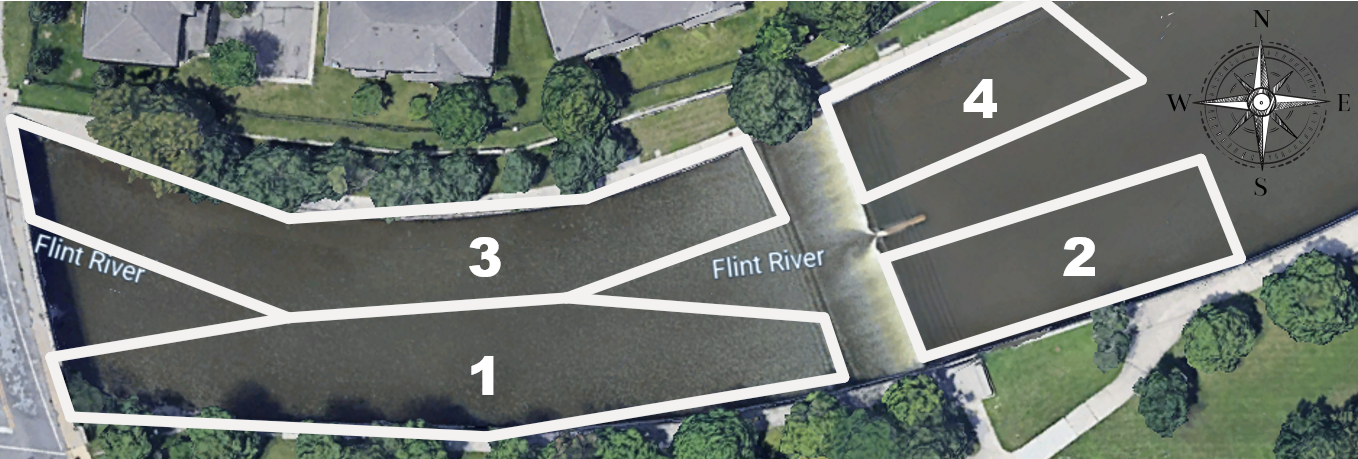
\includegraphics[width=\textwidth]{Img/Site_Map.png} \\
    \large
    \textbf{Site Map} \\
}

%%% Diversity %%%%%%%%%%%%%%%%%%%%%%%%%%%%%%%%%%%%%%%%%%%%%%%%%%%%%%%%%%%%%%%%%%
\headerbox{Diversity}{name=box10, column=1, row=0}{
  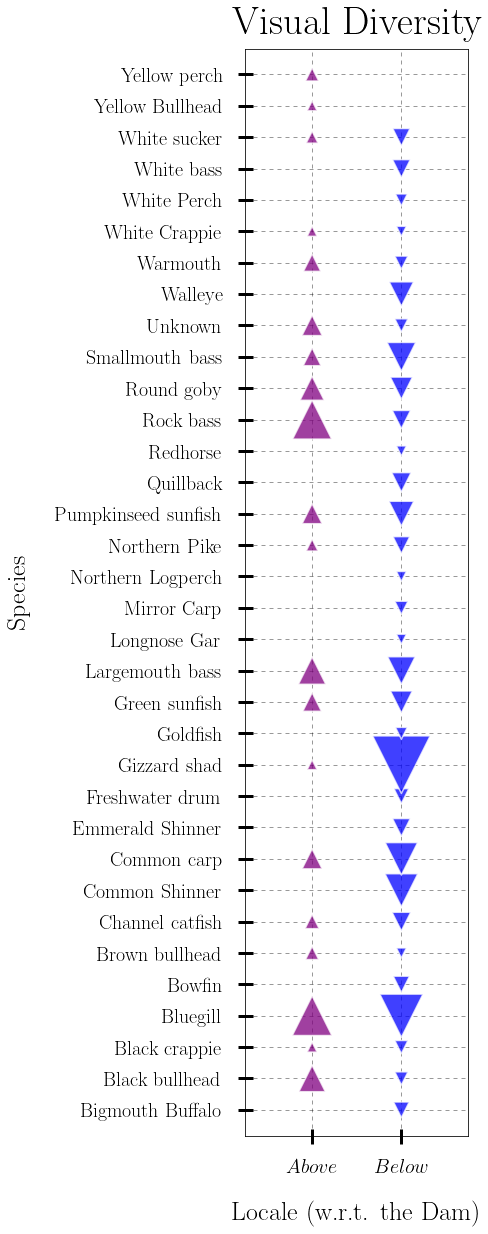
\includegraphics[width=.9\textwidth]{Img/Diversity_Bubble_Plot.png} \\

  In this figure we compare catch rates between sites $1/3$ below the dam, and sites $2/4$ above the dam. 
  Notable differences show much higher catch rates of gizzard shad below the dam and rock bass above the dam.
}

%%% Analysis %%%%%%%%%%%%%%%%%%%%%%%%%%%%%%%%%%%%%%%%%%%%%%%%%%%%%%%%%%%%%%%%%%%%%
\headerbox{Analysis}{name=box20, column=2, row=0}{

  \hspace{5mm}
  Using Simpson's Diversity Index we compared species diversity above and below the dam. 
  We computed relative index values of $0.77$ at site $1$, $0.77$ at site $2$, $0.48$ at site $3$, and $0.72$ at site $4$. \\
  \begin{center}
    Simpson's Diversity Index 
    $ \displaystyle D = 1 - \frac {\sum n(n-1)} {N(N-1)} $ \\
  \end{center}
  Values close to $1$ indicate perfect species diversity while values close to $0$ indicate single species domination. \\
}

%%% Descriptions %%%%%%%%%%%%%%%%%%%%%%%%%%%%%%%%%%%%%%%%%%%%%%%%%%%%%%%%%%%%%%%%%%%%%
\headerbox{}{name=box30, column=3, row=0}{

  \hspace{5mm}

}

\end{poster}
\end{document}
